The algorithms from the previous section were compiled into a library for data matching and exploration.
There are several reasons for this design choice, which become obvious when we look at the alternative.
Another possibility would have been to create services that process one or more dataframes with all the available functions
and return the result.
However, a library is much more flexible.

First of all, by storing functions in a library and calling them from the matcher service, we offer the user the option to
only select the relevant functions for the task at hand.
This is important because, while we can determine when a function is technically inapplicable (for example, two-sample T-test
only works on continuous, numerical series), there are many ambiguous scenarios where trying out different combinations of
functions on the same dataframes can provide noteworthy results.

Second of all, it is a question of performance.
Fig~\ref{fig:data_matching_library_function_types} is one layer of the structure of our data matching library, showcasing
different types of functions based on how they interact with the data.

\begin{figure}[h]
    \centering
    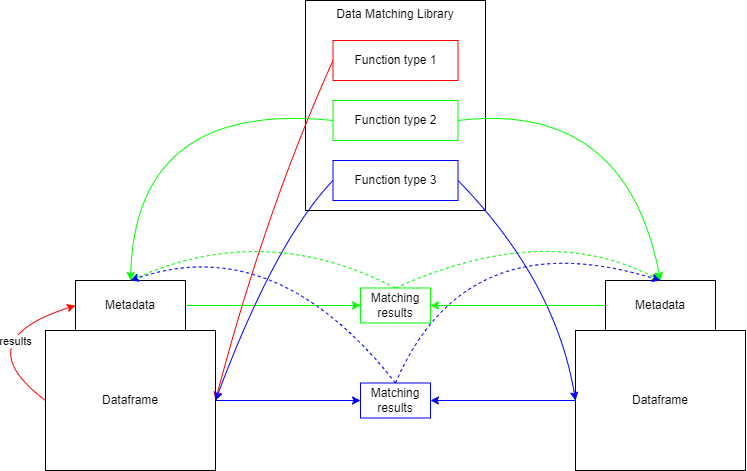
\includegraphics[width=12cm]{figures/data_matching_library/data_matching_library}
    \caption{Data matching library function types}
    \label{fig:data_matching_library_function_types}
\end{figure}

This is just one possible classification, but it is useful for identifying performance differences and deciding how to
handle results.
The first function type (red) is applied on the dataframe and generates results which should be included in the metadata.
These are metadata builder functions such as the Augmented Dickey-Fuller Test for stationarity, the formula for calculating
the percentage of numerical values in a column, and the formula for calculating the continuity factor of a column.
These results are expensive to calculate and, therefore, should be included in the metadata, as they will be used in further
exploration and matching algorithms.

The second function type (green) uses the metadata of two dataframes to generate similarity or correlation estimates.
These functions help create a network of data structures and reveal information about seemingly unrelated pieces of data.
They are computationally efficient, because they only use metadata, without accessing the dataframe rows, so, at least
in theory, we could compute these results as often as we need them.
However, it is still useful to store some of them in the metadata, for example, similarity percentages between the columns
of two particularly related dataframes, as they may be displayed to the user in different formats or sent for further processing.
Examples of functions of type two include all name matching functions, comparisons of column aggregates (such as minimum, maximum,
and mean values), and comparisons of the results of type one functions (continuity, numerical percentage and stationarity).

Finally, the third function type (blue) uses the actual rows of a dataframe to generate similarity estimates.
These results are expensive to compute, and therefore should be stored in the metadata and reused from there instead of
calculated from scratch whenever possible.
Functions of type three include matching identical rows, calculating the Pearson coefficient, performing the two-sample t-test,
and the Dynamic Time Warping algorithm.

The question that remains is how to store matching results in the metadata.
Do we store them in the metadata files attached to both dataframes or only in one of them?
And do we store every result for every single column?
The answer is: it depends.
If we are exploring the data from the perspective of one test dataframe, which we want to know more about, then it is
sufficient to store matching results only in its metadata file.
For example, we might want to store the top N most similar columns to each column in our dataframe, after exploring the entire
data catalog.
However, there are situations in which we must store results in both metadata files of dataframes under comparison, because
the obtained percentages might not be mutual.
For example, when determining the best column match in dataframe B for every column in dataframe A, the results may differ
if we swap the dataframes around.
We must also pay attention to how fast the obtainable information in our data catalog grows.
Storing every similarity percentage between any two columns in any two dataframes is not feasible in the long run, as the
space complexity of such an endeavor is quadratic on the total number of columns in the data catalog.
The solution is to identify dataframes of interest where we temporarily extend the metadata with column relationships.
Use cases where we exemplify these techniques will be present in the following chapter.

One final component that we need in order to utilize this library is an interface that can receive all relevant parameters
and run one of the matching functions in the library.
The list of parameters must include the name of the function that should be called, the metadata information of the two columns
that we are trying to match (if the function performs computation on two columns), the columns themselves (if the function needs
to access the data rows), and the metadata information of the two dataframes to which the columns belong.
The last parameter is relevant because storing a column relationship in a metadata file requires some kind of identifier for
the second column beyond its name.
For this, we can use the hash of the file containing its dataframe.
The concept of hashing large files and the various performance considerations behind it will be discussed in a different chapter.
